\documentclass{ctexart}

\usepackage{amsmath}
\usepackage{booktabs}
\usepackage{graphicx}
\usepackage{caption}
\usepackage{subfigure}

\begin{document}
\tableofcontents

\begin{abstract}
这份文档的目的是收集和整理摄影相关知识和目标相机的相关知识与特性,以帮助确定摄影设备的购买决策。

关于摄影部分的知识,目前计划中的内容包括。
\begin{itemize}
    \item 摄影器材参数概念:焦距、快门、光圈、ISO等;
    \item 摄影概念:景深、果冻效应等
\end{itemize}
对于每款相机,目前关心的特性主要包括:
\begin{itemize}
    \item 基本信息:品牌,上市时间,价格走势;
    \item 关键性能参数:画幅,ISO,像素,光圈,对焦,镜头卡口等
\end{itemize}
\end{abstract}

\section{相机基础知识}

\subsection{单反和无反}
这里的"反"指的是反光镜,即相机内部是否存在反光镜。大多数情况下,数码单反相机与过去的胶片机采用相同的设计。如图~\ref{fig_single_lens_reflex_vs_mirrorless}所示。相机机身内的一面镜子可以反射进入镜头的光线,透过棱镜进入取景器,这样你就可以预览你的照片。 当你按下快门按钮时,镜子翻转起来,快门打开,光线照射到图像传感器上,传感器捕捉到最终的图像。
\begin{figure}
    \centering
    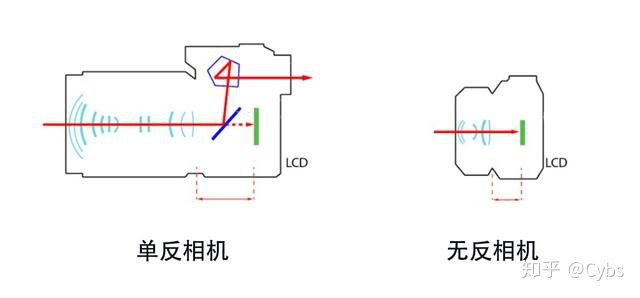
\includegraphics[width=.8\textwidth]{imgs/camera_single_lens_reflex_mirrorless.jpg}
    \caption{单反相机与无反相机内部对比。}
    \label{fig_single_lens_reflex_vs_mirrorless}
\end{figure}
在无反相机中,顾名思义,它是没有反光镜的,光线通过镜头直接进入图像传感器,传感器捕捉图像,我们可以通过在后屏幕上预览照片和取景。

从趋势来看,主要厂商都将大部分精力投向了无反机器,因此无反机器是目前的主流形式。

\subsection{画幅~\cite{frame}}
画幅(frame)可以理解为相机感光元件面积的大小,按照画幅大小区分,有:
\begin{itemize}
    \item 大画幅,骨灰级玩家;
    \item 中画幅,哈苏、飞思、富士等都有相关产品,多用于商社摄影,对画质要求极高的场合;
    \item 全画幅(full frame),通常说的135画幅;
    \item ASP-C画幅,即半画幅,多用于入门机型;
    \item M43画幅,富士、奥林巴斯还有相关产品;
    \item 一英寸,常见于卡片机、摄像机
    \item 其他,更小的画幅一般用于手机中的感光原件
\end{itemize}
图~\ref{fig_frame_comparison}展示了不同画幅大小的对比。
\begin{figure}[h]
    \centering
    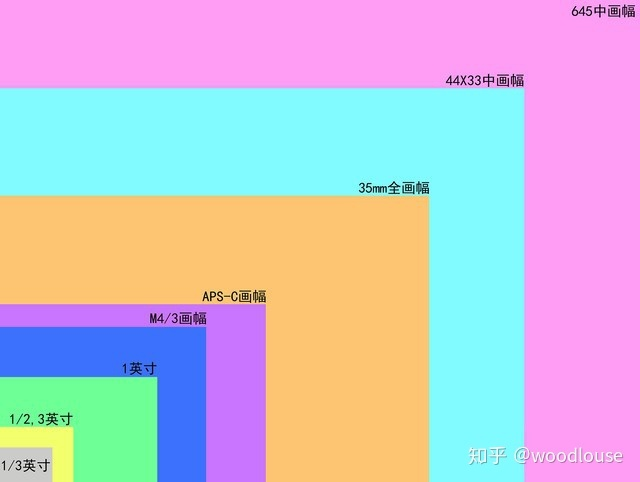
\includegraphics[width=.60\textwidth]{imgs/frame.jpeg}
    \caption{不同尺寸画幅的对比。}
    \label{fig_frame_comparison}
\end{figure}
画幅直接影响拍摄视野、光圈、焦距等关键参数。用于全幅的镜头可以装在半幅机器上,但焦距需要转换;但半幅机器的镜头不能用在全幅机器上。全幅机器的焦距用在半幅机器时,实际的等效焦距需要乘以1.5。图~\ref{fig_frame_photo}展示了不同画幅对成像大小和视野的影响。
\begin{figure}[!h]
    \centering
    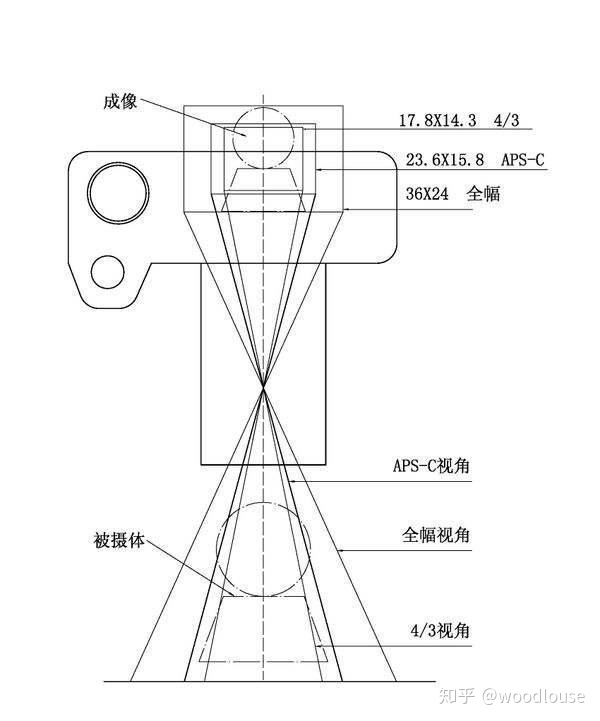
\includegraphics[width=0.5\textwidth]{imgs/frame_photo.jpg}
    \caption{不同画幅对于成像的影响分析。}
    \label{fig_frame_photo}
\end{figure}
可以很明显地发现,传感器面积变小,会导致相比于全幅,成像的视野变小。换句话说,半幅机器得到的视野是全幅机器经过裁切的,因此也相当于将镜头的焦距变大了,而如果希望获得相同的视野,就需要增大拍摄距离。

\subsection{焦距~\cite{focal_length_shutter_etc}}
\begin{figure}[h!]
    \centering
    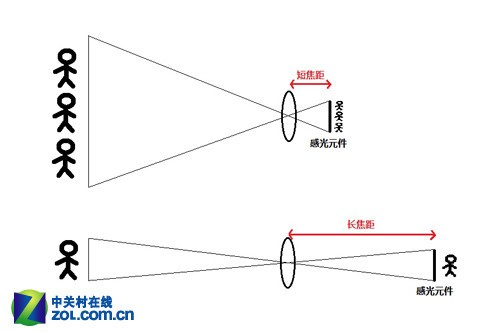
\includegraphics[width=.8\linewidth]{imgs/focal_length.jpg}
    \caption{不同焦距对成像的影响。小焦距下,可以拍摄更小的范围,而大焦距下,可以更好的放大远处的物体。}
    \label{fig_focal_length}
\end{figure}
焦距的英文是focal length,是指从镜头的光学中心(主点)到成像面(焦点)的距离,一般用符号$f$表示,单位是$mm$(毫米)。这一距离越短,则越能拍摄更广的范围(广角);此距离越长,则越能将远处的物体放大(长焦)。如图~\ref{fig_focal_length}所示。

镜头的焦距决定拍摄成像的大小、视场角大小、景深以及画面的透视。对于一定距离下的拍摄物体,焦距越短,则物体成像越小,拍摄范围越大;焦距越大,则物体成像越大。对于一24x46mm的全画幅相机,通常把焦距分为超广角、广角、标准、中焦、长焦和望远。图~\ref{fig_focal_length_category}的表展示了长焦相机焦距分类。
\begin{figure}[h!]
    \centering
    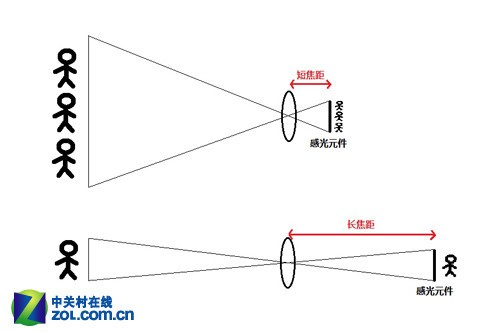
\includegraphics[width=.8\linewidth]{imgs/focal_length.jpg}
    \caption{焦距的分类。}
    \label{fig_focal_length_category}
\end{figure}

广角和长焦有着各自的优势。广角镜头虽然有着广阔的拍摄范围,但却也有明显的镜头畸变,所以在拍摄人像上并不给力。而长焦镜头虽然可以将远处的物体拉进,十分适合特写,但却不能拍摄较大的场面。

相机镜头可以分为变焦镜头和定焦镜头。变焦镜头表示焦距可以在一定范围内变化,例如18-105mm即表示镜头可以支持的焦距范围,使用长焦数值除以广角数值,就是镜头的变焦倍率,例如$\frac{105}{18}=5.8$,即镜头的变焦倍率为5.8;同时3.5-5.6表示镜头在广角和长焦端的最大光圈。一般来说,在变焦镜头中,变焦倍率很大的镜头虽然适用范围广,饭成像效果可能不如变焦倍率小一些的镜头。变焦倍率在3倍左右的镜头一般成像效果最好。

\subsection{ISO}
ISO即感光度,可以理解为对光线的敏感程度,ISO数字越大代表感光度越高,感光度越高,则对光线更敏感,即相同进光量的情况下画面越亮;但感光度过高时,画面的噪点会增多,影响画面质量。

\begin{figure}[h!]
    \centering
    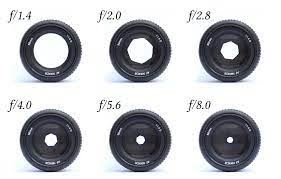
\includegraphics[width=.8\linewidth]{imgs/aperture_size.jpg}
    \caption{不同光圈大小,左侧为大光圈f/1.4,右侧是小光圈f/16。}
    \label{fig_aperture_size}
\end{figure}

\subsubsection{光圈}
光圈,英文名称Aperture,光圈控制着快门按下时孔径的大小,即可以控制进光量。光圈数值一般用${f/x}$表示,x数字越小,则光圈越大,即进光量越大。图~\ref{fig_aperture_size}展示了一个例子。

从数学角度来说,可以使用光通量表示进光量的大小。假设用$Y$表示光通量,用$D$表示镜头透镜孔径的大小,单位为$mm$(毫米),则可以将其定义为:$Y=\frac{D}{f}$。
直观来看,孔径$D$越大,焦距越小,则光通量越大。而一般镜头标注的光圈值$F$是光通量的倒数,即$F=\frac{f}{D}$。例如50mmm F/1.8的镜头,可以计算出孔径$D=\frac{f}{F}=27mm$。
由于镜头的焦距通常不能小于镜头卡口到焦平面的距离(即法兰距离),而镜头口径不能大于镜头卡口直径, 所以光圈值$F$有一个最小值,即焦距$f$取最小,且孔径$D$取最大值。由于光通量与孔径的平方成正比(将孔径视作原型,光通量与原型面积成正比),因此,当孔径增大一倍,则光通量变为原来的$\frac{1}{4}$。换句话说,如果镜头焦距不变,光圈值$F$增大一倍,则光通量减少为原来的$\frac{1}{4}$。
所以,在镜头上,相邻的两档之间光圈值为$\sqrt{2}$倍的关系,即光通量为2倍关系。图~\ref{fig_aperture_math}展示了上面介绍的概念。
\begin{figure}[h!]
    \centering
    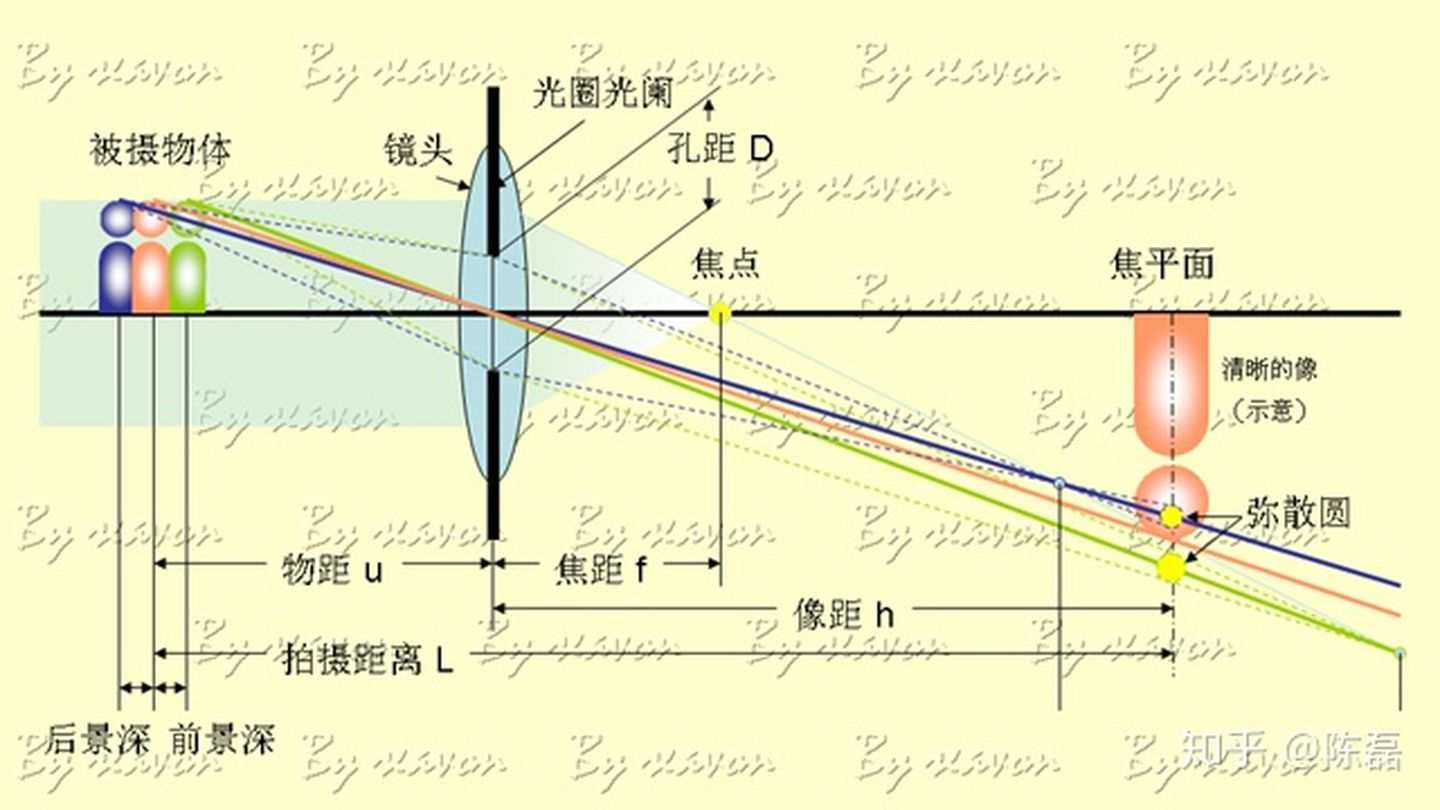
\includegraphics[width=.8\linewidth]{imgs/aperture_math.jpg}
    \caption{镜头孔距、焦距等的关系示意图。}
    \label{fig_aperture_math}
\end{figure}

光圈主要可以影响两个因素:景深和亮度。一般需要很好背景虚化的效果时,需要大光圈;此外,光线较暗的情况下,也需要大光圈。

\subsubsection{快门}
快门:英文名称Shutter,快门就是控制感光原件曝光时间的长短,即控制进光量,快门速度一般用$\frac{1}{x}$s来表示,表明快门打开的持续时间,$x$越大则时间越短,即快门越快。一般来说,宽门速度块则进光时间短,亮度低。此外,由于在快门时间内在持续曝光,所以如果相机不稳时,在较长的快门时间下就容易出现模糊的情况。一般来说,有一个安全快门的说法,即快门不低于焦距的倒数。

按照原理,快门可分为机械快门和电子快门一般来说,机械动作都有速度极限,常见的机械快门速度为$\frac{1}{4000}$s或$\frac{1}{8000}$s,在按下快门前,窗口不见光,而按下快门后,帘幕快速打开并关闭,从而使得窗口获得指定时间长短的见光机会。

而电子快门没有机械结构,它依靠对感光元件充电的控制起到快门的作用,快门速度可以轻松达到$\frac{1}{10000}$s甚至更高。理论上,有更高的快门速度,就可以配合更大的光圈。然而,电子快门也有一些缺点。首先是由于感光原件进行逐行扫描,如果拍摄速度比较快的运动物体就有可能会有果冻效应。

快门、光圈与ISO是控制曝光的3个基本因素~\cite{iso_aperture_shutter},图~\ref{fig_iso_aperture_shutter}形象地展示了3者对最终成像的影响。

\begin{figure}[h!]
    \centering
    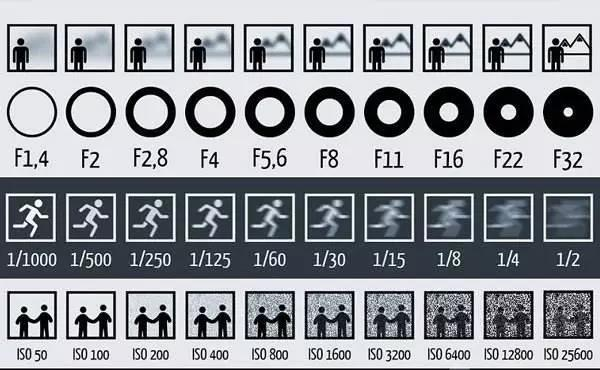
\includegraphics[width=.7\linewidth]{imgs/iso_aperture_shutter.jpg}
    \caption{光圈、快门速度与ISO对最终成像的影响。}
    \label{fig_iso_aperture_shutter}
\end{figure}

\section{摄影基础知识}

\subsection{景深~\cite{depth_of_field}}
景深与多种因素相关,包括光圈、焦距、画幅等。景深可以直观理解为摄影机拍摄的物体的深度,景深越深,拍摄的物体越模糊,景深越浅,拍摄的物体越清晰。
景深的由来可以参考图~\ref{fig_aperture_math}。在图中,被摄物体中的黄色任务满足焦距,成像恰好落在焦平面上。而对于不在合焦距离上的物体,例如绿色和蓝色任务,则会在焦平面上形成一个与镜头孔径形状类似的光斑。
这个光斑称为弥散圆。当光斑越大时,则物体成像越模糊,这就是景深的由来。景深可以理解为,在合焦距离的前后多大范围内,弥散圆的大小小于容许值(光斑小于容许弥散圆)。
通常情况下,容许弥散圆的大小是画幅对角线长度的$\frac{1}{1500} - \frac{1}{1000}$。

基于图~\ref{fig_aperture_math},我们可以推断出,在确定的镜头和相机下,即焦距$f$、孔径$D$、光圈值$F$,容许弥散圆大小$\delta$确定,
设和焦物体物距为$u$,推测满足要求的最大景深$\Delta u$:
根据光学基本知识,我们有:
\begin{equation}
    \frac{1}{u}+\frac{1}{h} = \frac{1}{f}
\label{eq_fuh}
\end{equation}
简单变形后,可得:
\begin{equation}
    h = \frac{uf}{u-f}
    \label{eq_h}
\end{equation}
因此,前景深$\Delta h$可以表示为:
\begin{equation}
    \Delta h = \frac{\Delta u f^2}{(u-\Delta u -f)(u-f)}
    \label{eq_deltah}
\end{equation}
注意,前景的物距小于u,而相距大于h。此时存在公式:
\begin{equation}
    \frac{\delta}{D} = \frac{\Delta h}{h+\Delta}
    \label{eq_delta_div_d}
\end{equation}
将公式~\ref{eq_h}和公式~\ref{eq_deltah}带入公式~\ref{eq_delta_div_d}:
\begin{align}
    \frac{\delta}{D} &= \frac{\delta uf}{(u-f)(u-\Delta u)} \\
    \Delta u &= \frac{\delta u(u-f)}{\delta(u-f)+(Df)}
    \label{eq_delta_u}
\end{align}
又由于$D=\frac{f}{F}$,带入公式~\ref{eq_delta_u}:
\begin{equation}
    \Delta u = \frac{\delta u(u-f)}{\delta(u-f)+\frac{f^2}{F}}
\end{equation}
类似的,对于后景深$\Delta u^{'}$,其物距大于u,像距小于h,此时有公式:
\begin{equation}
    \frac{\delta}{D} = \frac{\Delta h}{h-\Delta h}
\end{equation}
类似地,最终可得:
\begin{equation}
    \Delta u^{'} = \frac{\delta u(u-f)}{\frac{f^2}{F}-\delta(u-f)}
\end{equation}
注意,前景深$\delta u$与后景深$\delta u^{'}$的差异仅在于分母,由于$u>f$,因此$\delta u^{'}>\delta u$。
即在同一场景内,在满足最大弥散圆情况下,后景深会大于前景深,也就是背景的虚化会比前景要好。另外,由于一般情况下有$u>>f$,且$\delta$很小,因此:
\begin{equation}
    \delta u = \frac{\delta u^{2}F}{f^{2}}
    \label{eq_delta_u_expro}
\end{equation}
根据公式~\ref{eq_delta_u_expro},我们可以知道:
\begin{itemize}
    \item 固定镜头焦距与光圈的情况下,物距越近,景深越小
    \item 固定镜头焦距与物距情况下,光圈值F越小,景深越小
    \item 在一定的物距和光圈值F下,焦距约大,景深越小
\end{itemize}
最后,由于容许弥散圆的大小$\delta$与感光元件尺寸成正比,而等效焦距也与感光元件尺寸成正比,因此对于不同的相机,在通用等效焦距和光圈情况下,拍摄同一个物体,感光元件尺寸越小,景深越小(分母为焦距的平方),且景深与感光元件尺寸成反比。
因此,手机的景深效果远不如全画幅相机。

\subsection{果冻效应~\cite{rolling_shutter}}
果冻效应(rolling shutter)是拍摄中作品中出现的一种被摄物体发生形变的现象。图~\ref{fig_rolling_shutter_exp}展示了2幅果冻效应的实例。
\begin{figure}[htbp]
    \centering
    \subfigure[果冻效应示例1]{
        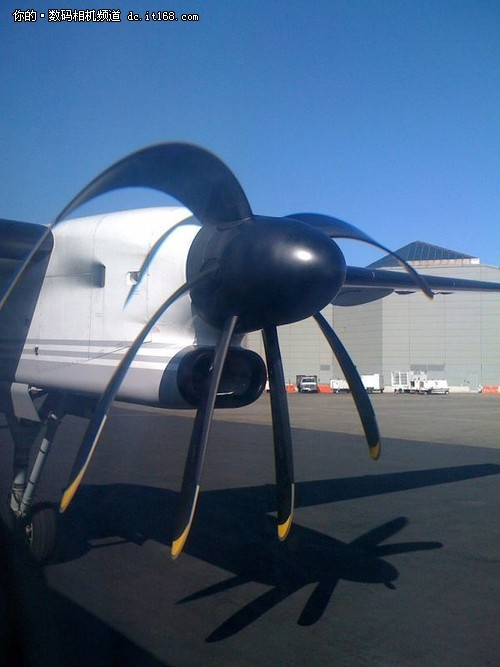
\includegraphics[width=.45\textwidth]{imgs/rolling_shutter_1.jpg}
    }
    \subfigure[果冻效应示例2]{
        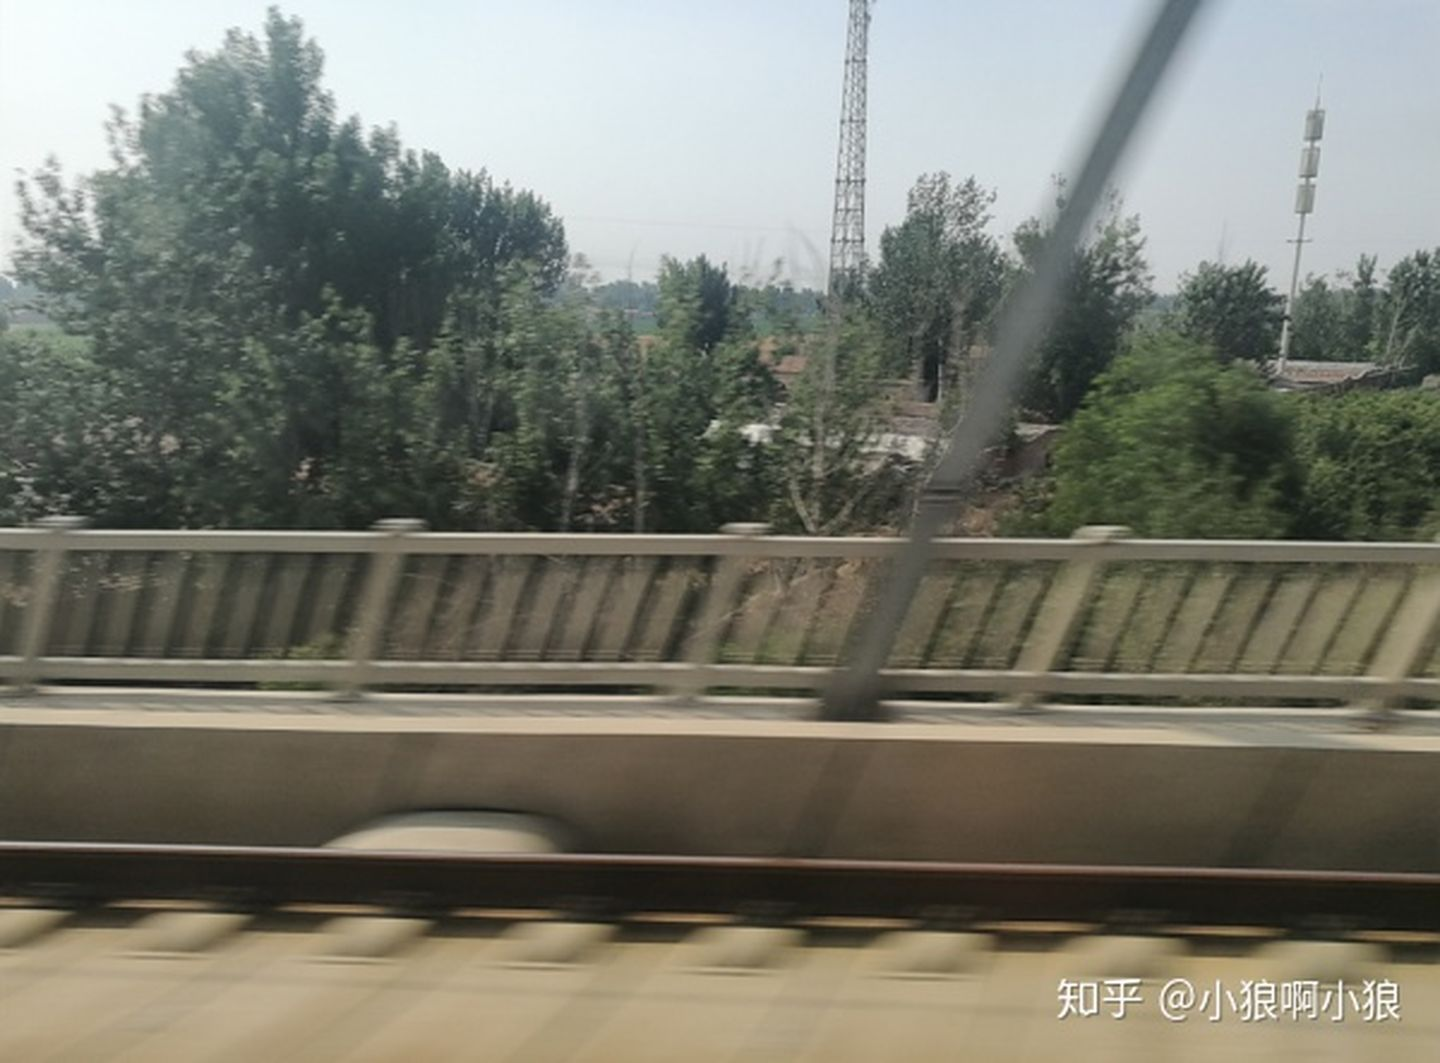
\includegraphics[width=.45\textwidth]{imgs/rolling_shutter_2.jpg}
    }
    \caption{果冻效应示例。高速运动的物体在照片中出现了明显的形变。}
    \label{fig_rolling_shutter_exp}
\end{figure}
果冻效应出现的原因与快门的原理紧密相关。快门一般可以分为机械快门和电子快门。果冻效应大多出现在电子快门的设备上。根据传感器的工作方式,可以将快门分为全局快门和卷帘快门。
全局快门就是在曝光的同一时间,传感器上的所有像素同时接受光源,再转化成电子信号。因此传感器记录的是被摄物体在同一时刻的形态,所以对抓拍高速移动的物体很有优势。全局快门一般用在以CCD为感光材料的设备上。
但是由于采用了全局快门后,传感器上的每一个像素的采光原件都要同时对数据进行转换,所以就增加了单个像素上采光原件的数目,导致单个像素的体积变大(占用更大空间),所以相同面积下的像素数目就变少了。因此,采用全局快门方式曝光的传感器很难达到很高的像素。

为了提高像素,采用了卷帘门曝光方式的传感器就出现了,而这也是目前CMOS最常使用的一种曝光方式。CMOS的曝光过程可以大致理解为这样的顾聪:“断点(信号清零)-曝光-通电(光源转换电信号成像)”。而且CMOS的曝光过程采用的是从上至下逐行扫描的方式进行的,有些类似于机械快门的焦平面快门的工作方式,因此CMOS的这种工作方式被称为卷帘快门。
这种逐行扫描的工作方式,就是果冻效应,或者说形变产生的原因。

图~\ref{fig_rolling_shutter_right}展示了水平高速运动物体的成像过程。由于镜头成像左右相反,且上下颠倒,因此CD首先经过扫描成像,而当扫描到AB时,由于物体的运动,AB位置相对CD发生了变化。所以最终成像的结果是一个平行四边形,上边AB相对CD朝运动方向发生了倾斜。
图~\ref{fig_rolling_shutter_exp}可以看到路边的栅栏向后倾倒的原因就在于此。
\begin{figure}[h]
    \centering
    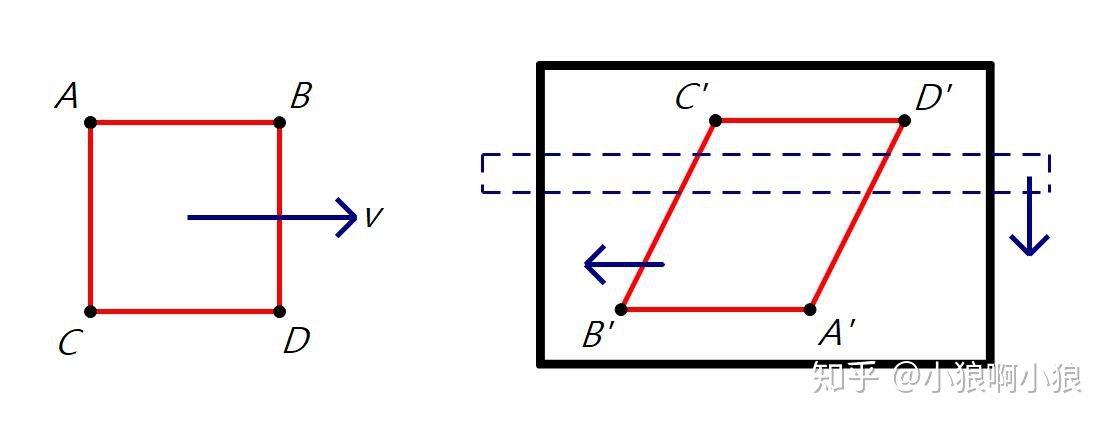
\includegraphics[width=.75\textwidth]{imgs/rolling_shutter_right.jpg}
    \caption{水平运动的物体由于果冻效应产生形变。}
    \label{fig_rolling_shutter_right}
\end{figure}
类似的,对于高速向上和向下运动的物体,便会有拉长效应和压缩效应,如图~\ref{fig_rolling_shutter_up_down}所示。
\begin{figure}[h]
    \centering
    \subfigure[向上运动物体的果冻效应分析]{
        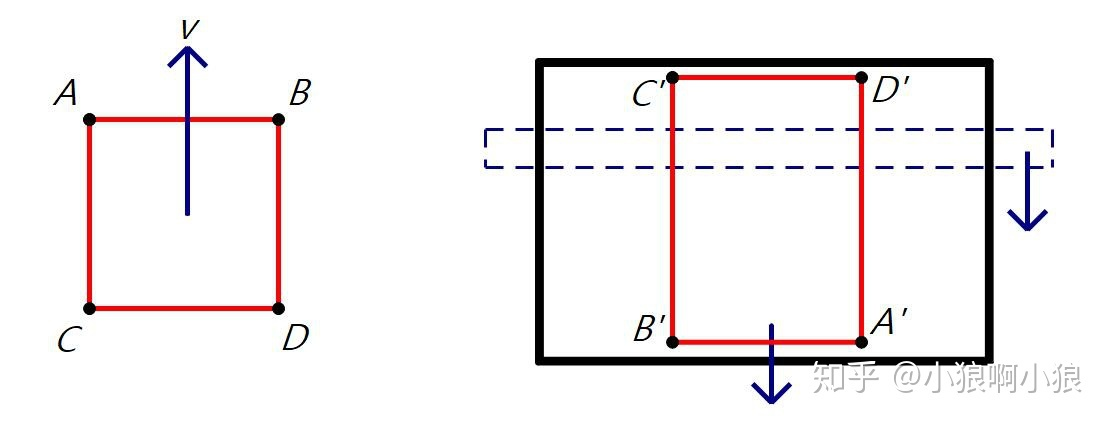
\includegraphics[width=.45\textwidth]{imgs/rolling_shutter_up.jpg}
    }
    \subfigure[向下运动物体的果冻效应分析]{
        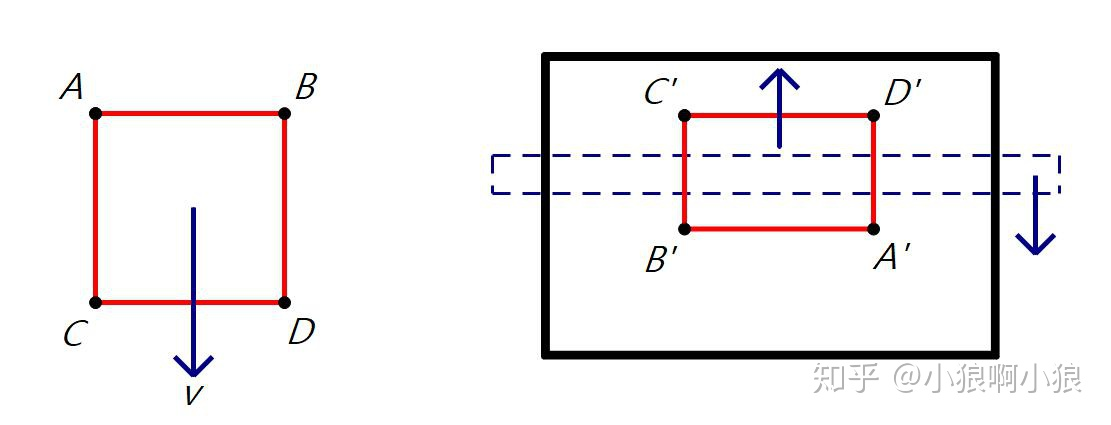
\includegraphics[width=.45\textwidth]{imgs/rolling_shutter_down.jpg}
    }
    \caption{上下运动物体的果冻效应。}
    \label{fig_rolling_shutter_up_down}
\end{figure}



\subsection{紫边效应\cite{chromatic_aberration1, chromatic_aberration2}}
紫边效应(purple fringing)是指在使用数码相机拍摄高反差、大背光的物体的照片中,物体边缘出现"紫边"的现象。
几乎所有的数码摄像摄影产品都存在这样的问题,差别仅在于程度问题。图~\ref{fig_purple_fringing}展示了建筑物边缘的紫边现象。
\begin{figure}[h]
    \centering
    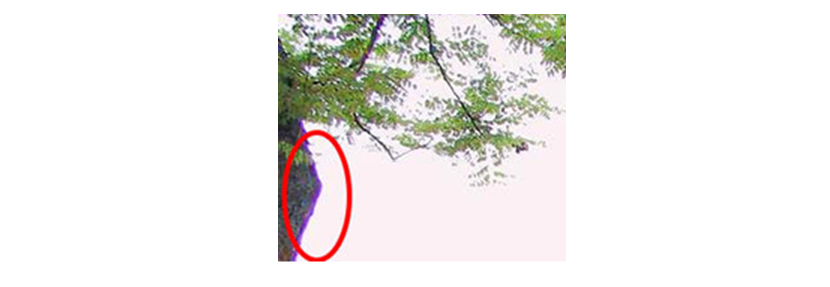
\includegraphics[width=.80\textwidth]{imgs/purple_fringing.jpg}
    \caption{拍摄高层背光建筑物时,边缘出现的紫边效应。}
    \label{fig_purple_fringing}
\end{figure}

事实上,关于紫边效应的原因还没有统一的定论。一种观点是认为,自编效应主要是由于镜头的色散引发的。色散是指镜头对不同波长的光线聚焦不在同一个焦平面,即不同波长的光线的焦距是不同的。对于波长较长的色光,透镜的折射率较低,由于透镜的焦距与折射率有关,所以它无法将光谱上的每一种色光都聚焦在光轴上的同一点。
这会导致在对焦时,部分色光可以精确聚焦在焦平面,而其他波长的色光则在焦平面形成光斑。这些色光混合后形成了其他颜色的边缘。
理论上,色散在影像的中央和边缘都可能发生,但由于边缘处光程较长,因此色散比较明显。

在实践中,长焦镜头、大光圈比较容易出现紫边效应。按照色散的解释,长焦镜头使得同样高度入射的光线,经过折射后光的间距大于普通镜头,所以色散现象更为严重。而大光圈下光会透射到镜头边缘,所以也比较容易形成色散。

另外一种分析认为,紫边主要的来源是数模转换算法的缺陷,因为在胶片时代,同样的镜头并不会出现紫边效应。首先,光是一种波,因此具有衍射(Diffraction)现象。当光通过一些小孔或者缝隙时,在物体的边缘会出现分散的现象。因此,对于高反差大背光的物体,强光通过边缘时,就已经出现了衍射现象,使得边缘部分的素质降低。衍射现象再加上目前CCD的原理导致了紫边。目前的CCD都是Mosaic遮罩式,CCD本身不感知色彩,通过CCD每个像素前的RGB路径,每个像素仅测量R、G、B其中一种原色的密度,再有相机内部软件进行彩色化插值处理,利用周边像素的信息插值出其他颜色。这个插值方式不可能完全还原真实颜色。在常用的BayerBattern滤镜排列中,R+B的组合最容易出现,而二者组合就形成了紫边的颜色。


\begin{figure}[h!]
    \centering
    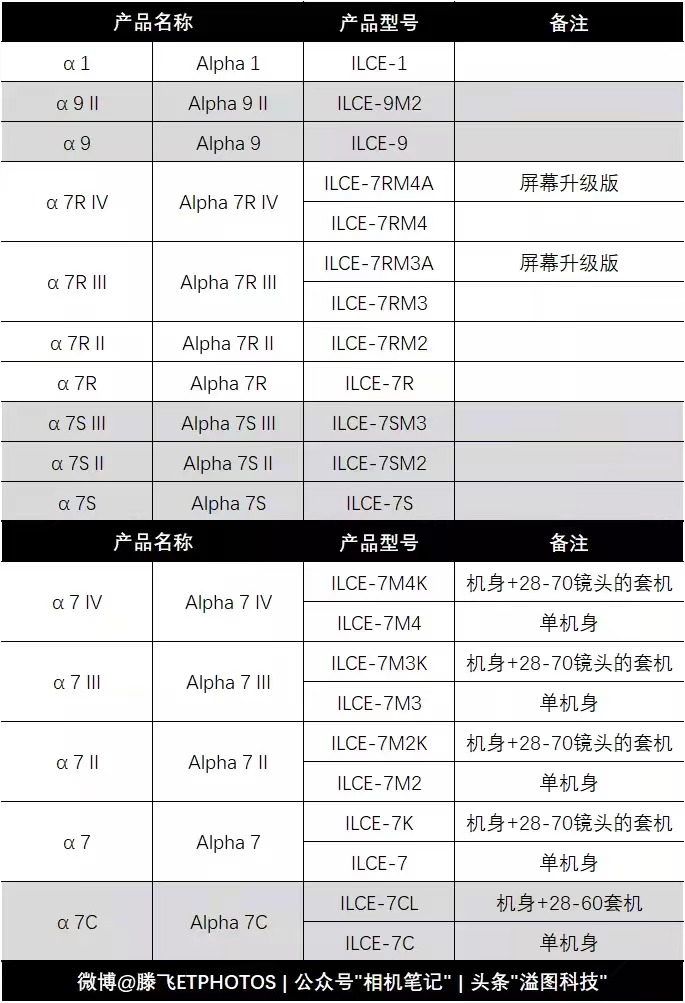
\includegraphics[width=.7\linewidth]{imgs/sony_product.jpeg}
    \caption{Sony微单产品}
    \label{fig_sony_products}
\end{figure}

\subsection{型号命名规则}

\subsubsection{Sony微单~\cite{sony_products_analysis}}
sony的主要微单产品可以参考图~\ref{fig_sony_products}。具体来说,每一款sony的全画幅微单产品都有产品名称和产品型号(SKU)两种称呼方式,而产品又可以细分为印刷版和书写板。

印刷版的产品名称是"$\alpha$"+1/7/9+(R|S|C)+II/III/IV;而书写版本的产品名称使用"Alpha"代替$\alpha$。产品型号与产品名称不同,它是"ILCE-"+1/7/9+(R|S|C)+M2/M3/M4+(A|K|L)。
其中,ILCE是“Interchangable Lens Camera with E mount(E卡口可更换镜头相机)”的缩写;在代表代数的数字后的R/S/C表示侧重不同的子系列。一般来说,R表示侧重画质的子系列,像素最高,目标为专攻相片的群体;S表示侧重高感,适用于视频拍摄;C则是入门系列。
以ILCE-7RM3A为例:
\begin{itemize}
    \item 7表明是$\alpha$7系列;
    \item R表示它是$\alpha$7系列中偏重画质的R子系列;
    \item M3表示它是$\alpha$7R中的第三代;
    \item A表示它是$\alpha$7RIII的小改宽,具体来说就是相对ILCE-7RM3改进了屏幕分辨率。
\end{itemize}
上面的分析也适用于ILCE-7RM4A。而对于ILCE-7M3K,后缀K表示它是机身+镜头的套机,这一规则也适用于ILCE-7K、ILCE-7M2K、ILCE-7M4K。


\section{非全画幅相机}
\subsection{Sony A6400}
\subsection{Sony A6600}

\section{全画幅相机}

\subsection{Sony $\alpha$7C}
也称为ILCE-7C,$\alpha$7C上市与2020年9月。

主要特性:
\begin{itemize}
    \item 小巧,轻便(重量?)
    \item 支持视频眼部对焦;
    \item 相比于$alpha$7 III具有更好的对焦、视频与网络功能
\end{itemize}
需要考虑的缺点
\begin{itemize}
    \item EVF放大倍率低
    \item 按键少,没有摇杆
    \item 没有全机械快门
\end{itemize}

\subsection{Panasonic LUMIX S5~\cite{panasonic_lumix_s5} }
全画幅微单,L卡口,上市时间为2020年9月,可以称为S1H的青春版。
\subsubsection{传感器}
\subsection{像素}
有效像素约2420w
\subsubsection{对焦}
相对较弱,静态物体对焦OK,但运动物体对焦较弱
\subsubsection{防抖}
6.5级的5轴防抖

其他特点包括:
\begin{itemize}
    \item 双原生ISO的全画幅传感器
    \item 6.5级的5轴防抖
    \item 支持多种视频记录规格,10biot 4K,以及104K 60fps
    \item 提供多种专业的视频辅助功能
    \item 良好的防抖性能
\end{itemize}
可能的缺点:
\begin{itemize}
    \item 连续对焦性能一般
\end{itemize}

\subsection{Sony $\alpha$7 IV~\cite{sony_alpha7_iv_announment}}
全画幅微单,E卡口,也称为ILCE-7M4,2021年10月发布,建议售价16999。它的定位是上一代全画幅相机$\alpha$7 III的继承者。相机采用了创新影像科技,包括:
\begin{itemize}
    \item 新研发的BIONZ XR影像处理器,与$\alpha$I一致
    \item 基于旗舰微单$\alpha$I的先进自动对焦技术
    \item 新的全画幅背照式Exmor R CMOS影像传感器
\end{itemize}
\subsubsection{传感器}
全新全画幅背照式Exmor R CMOS影像传感器。
\subsection{像素}
有效像素3300w。
\subsubsection{对焦}
与$\alpha$I一致的自动对焦技术,在10张/s*2的高速连拍下实现AF/AE跟踪。
对焦基于759个相位检测对焦点。
支持照片和视频下的人眼对焦、鸟类与动物眼部实时追踪。
相比$\alpha$7 III,人脸和人眼检测精度提升约30$\%$。
\subsubsection{感光}
ISO 50-204800,在低感光度下具备16级动态范围
\subsubsection{防抖}
内置5轴防抖,实现5.5级防抖效果。
\subsubsection{屏幕、取景器与控制菜单}
3.0寸103w点侧翻式LCD触摸屏。
368w点OLED Quad-VGA取景器。


\subsection{Sony A7C}
全画幅微单,E卡口,上市时间2020年9月,SKU为ILCE-7C,价格xxxx。
相对ILEC-7M3,有更好的对焦、视频与网络功能,也是最小巧的、内置5轴防抖的全画幅微单。
\subsection{Sony A7M III}
全画幅微单,E卡口,上市时间2018年2月,SKU为ILCE-7M3,价格xxxx。
\subsection{Sony A7R III(A)}
全画幅微单,E卡口,7RM3与2017年10月上市,SKU为ILCE-7RM3,7RM3A改进款上市时间2012年4月,SKU为ILCE-7RM3A,基于前一代改进了屏幕,价格xxxx。
\subsection{Sony A7S III}
全画幅微单,E卡口,上市时间2020年7月,SKU为ILCE-7SM3,定价23999。

\subsection{Nikon Z5}
全画幅微单,Z卡口,发布于2020年7月,机身万元以内。主要特点包括:
\begin{itemize}
    \item 与Z6、Z7系列基本相同的操控体验
    \item 同价位中优秀的画质
\end{itemize}
需要考虑的问题包括:
\begin{itemize}
    \item 连拍速度较低
    \item 4K视频实用性较差
\end{itemize}
\subsection{Nikon Z6}
\subsection{Canon EOS RP}


\bibliographystyle{plain} % We choose the "plain" reference style
\bibliography{sample} % Entries are in the sample.bib file

\end{document}